%%%%%%%%%%%%%%%%%%%%%%%%%%%%%%%%%%%%%%%%%
% Beamer Presentation
% LaTeX Template
% Version 1.0 (10/11/12)
%
% This template has been downloaded from:
% http://www.LaTeXTemplates.com
%
% License:
% CC BY-NC-SA 3.0 (http://creativecommons.org/licenses/by-nc-sa/3.0/)
%
%%%%%%%%%%%%%%%%%%%%%%%%%%%%%%%%%%%%%%%%%

%----------------------------------------------------------------------------------------
%	PACKAGES AND THEMES
%----------------------------------------------------------------------------------------

\documentclass{beamer}

\mode<presentation> {

% The Beamer class comes with a number of default slide themes
% which change the colors and layouts of slides. Below this is a list
% of all the themes, uncomment each in turn to see what they look like.

%\usetheme{default}
%\usetheme{AnnArbor}
%\usetheme{Antibes}
%\usetheme{Bergen}
%\usetheme{Berkeley}
%\usetheme{Berlin}
%\usetheme{Boadilla}
%\usetheme{CambridgeUS}
%\usetheme{Copenhagen}
%\usetheme{Darmstadt}
%\usetheme{Dresden}
%\usetheme{Frankfurt}
%\usetheme{Goettingen}
%\usetheme{Hannover}
%\usetheme{Ilmenau}
%\usetheme{JuanLesPins}
%\usetheme{Luebeck}
%\usetheme{Madrid}
%\usetheme{Malmoe}
%\usetheme{Marburg}
%\usetheme{Montpellier}
%\usetheme{PaloAlto}
%\usetheme{Pittsburgh}
%\usetheme{Rochester}
%\usetheme{Singapore}
%\usetheme{Szeged}
\usetheme{Warsaw}

% As well as themes, the Beamer class has a number of color themes
% for any slide theme. Uncomment each of these in turn to see how it
% changes the colors of your current slide theme.

%\usecolortheme{albatross}
%\usecolortheme{beaver}
%\usecolortheme{beetle}
%\usecolortheme{crane}
%\usecolortheme{dolphin}
%\usecolortheme{dove}
%\usecolortheme{fly}
%\usecolortheme{lily}
%\usecolortheme{orchid}
%\usecolortheme{rose}
%\usecolortheme{seagull}
\usecolortheme{seahorse}
%\usecolortheme{whale}
%\usecolortheme{wolverine}

%\setbeamertemplate{footline} % To remove the footer line in all slides uncomment this line
%\setbeamertemplate{footline}[page number] % To replace the footer line in all slides with a simple slide count uncomment this line

%\setbeamertemplate{navigation symbols}{} % To remove the navigation symbols from the bottom of all slides uncomment this line
}

\usepackage{graphicx} % Allows including images
\usepackage{booktabs} % Allows the use of \toprule, \midrule and \bottomrule in tables
\usepackage{amsmath}

\AtBeginSection[]
{
   \begin{frame}
       \frametitle{Outline}
       \tableofcontents[currentsection]
   \end{frame}
}

%----------------------------------------------------------------------------------------
%	TITLE PAGE
%----------------------------------------------------------------------------------------

\title[Sum of Divergent Series]{Sum of Divergent Series} % The short title appears at the bottom of every slide, the full title is only on the title page

\author{Haoen CUI} % Your name
\institute[Uptake] % Your institution as it will appear on the bottom of every slide, may be shorthand to save space
{
Uptake Math Club Lightning Talk
% Your institution for the title page
% Your email address
}
%\date{\today} % Date, can be changed to a custom date
\date{February 15 \& 22, 2019}

\begin{document}

\begin{frame}
\titlepage % Print the title page as the first slide
\end{frame}

%----------------------------------------------------------------------------------------
%	PRESENTATION SLIDES
%----------------------------------------------------------------------------------------

%------------------------------------------------
\section{Motivating Examples} 
%------------------------------------------------

\begin{frame}
\frametitle{Motivating Examples} 
\begin{figure}

\includegraphics[width=\linewidth]{success_kid.jpg}
\end{figure}
\end{frame}

%------------------------------------------------

\subsection{Recap from Last Time} 

\begin{frame}
\frametitle{Convergence of Power Series}

Last time, \textcolor{cyan}{@willdiesel} talked about the following Maclaurin series (i.e. Taylor series expanded at zero)
$$ \frac{1}{1-x} = 1 + x + x^2 + x^3 + \cdots = \sum_{n=0}^{\infty} x^n $$

\begin{itemize}
    \item \textcolor{cyan}{@bernie} asked about \alert{convergence} (which is $ |x| < 1 $) 
    \item But, what does it mean when we write $ \sum_{n=0}^{\infty} x^n = \textit{value} $ ?
    \begin{itemize}
        \item Is ``$=$'' a mathematical equivalence symbol or an assignment operator? 
    \end{itemize}
\end{itemize}

\end{frame}

%------------------------------------------------

\begin{frame}
\frametitle{Review of Summation of Real Numbers}

\begin{block}{Properties of Sum of Real Numbers}
\begin{itemize}
    \item \textbf{Commutativity}: For $ \forall x, y \in \mathbb{R} $, $x + y = y + x $
    \item \textbf{Associativity}: For $ \forall x, y, z \in \mathbb{R} $, $ (x + y) + z = x + (y + z) $ 
\end{itemize}
\end{block}

\begin{block}{Recursive Definition of $ \sum $ Symbol}
For $ \forall \{a_i\}_{i \in \mathbb{N}} \subset \mathbb{R} $ and $ \forall n \in \mathbb{N} $, define the summation symbol, 
$$ \sum_{i=1}^{n} a_i = a_n + \sum_{i=1}^{n-1} a_i 
\quad (\text{for } n > 1) \quad \text{ and } \quad 
\sum_{i=1}^{1} a_1 = a_1 $$
(Note: $ \infty $ is not a real number nor a natural number.)
\end{block}

\end{frame}

%------------------------------------------------

\subsection{Numberphile Video}

\begin{frame}
\frametitle{Sum of All Natural Numbers}

\href{https://www.youtube.com/watch?v=w-I6XTVZXww}{Numberphile Video: ASTOUNDING! $ 1 + 2 + 3 + \cdots = -\frac{1}{2} $} \\ 
\ \\
Consider the following sums
\begin{align*}
    S   &= 1 + 2 + 3 + 4 + 5 + 6 + \cdots \\ 
    S_1 &= 1 - 1 + 1 - 1 + 1 - 1 + \cdots \\ 
    S_2 &= 1 - 2 + 3 - 4 + 5 - 6 + \cdots
\end{align*}
We want to find $S$ and we establish $S_1$ and $S_2$ as intermediate steps. 

\end{frame}

%------------------------------------------------

\begin{frame}
\frametitle{Sum of All Natural Numbers (Cont.)}

First, we find the values of ``helper'' sums $S_1$ and $S_2$. 

\begin{block}{Claim 1 and 2: $ S_1 = \frac{1}{2} $ and $ 2 S_2 = S_1 \implies S_2 = \frac{1}{4} $}
Because the partial sums are $0, 1, 0, 1, \cdots$, so $\frac{1}{2}$ is sort of the average, hence $ S_1 = \frac{1}{2} $. Furthermore, 
\begin{alignat*}{3}
2 S_2 &= S_2 && + && S_2 \\
      &= 1   && - && 2 + 3 - 4 + 5 - 6 + \cdots \\ 
      &      &&   && 1 - 2 + 3 - 4 + 5 - \cdots \\ 
      &= 1   && - && 1 + 1 - 1 + 1 - 1 + \cdots \\
      &= S_1 &&   &&
\end{alignat*}
\end{block}

\end{frame}

%------------------------------------------------

\begin{frame}
\frametitle{Sum of All Natural Numbers (Cont.)}

Next, we can fill the bridge to $S$. 

\begin{block}{Claim 3: $ S - S_2 = 4 S \implies S = -\frac{1}{12} $}
\begin{align*}
    S - S_2 = \quad &1 + 2 + 3 + 4 + 5 + 6 + \cdots \\ 
            -( &1 - 2 + 3 - 4 + 5 - 6 + \cdots) \\ 
            = \quad &0 + 4 + 0 + 8 + 0 + 12 + \cdots \\ 
            = \quad &4(1 + 2 + 3 + \cdots) \\ 
            = \quad &4S
\end{align*}
\end{block}

\end{frame}

%------------------------------------------------

\begin{frame}
\frametitle{Sum of All Natural Numbers (Cont.)}

But, the result doesn't follow along with the intuition 
$$ \{a_i\} \subset \mathbb{R}_{+} \implies \forall N \in \mathbb{N}, \sum_{i=1}^{N} a_i > 0 $$

What may go wrong? 
\begin{itemize}
    \item What is the definition of sum? 
    $$ \Sigma_{i=1}^{\infty} a_i = a_1 + a_2 + a_3 + \cdots \text{ is just a short hand notation} $$
    \item Can we shift terms in a series under summation? 
    \item Can we ignore all the zeros, despite the infinite amount? 
    \item Is summation a linear operator? 
\end{itemize}

\end{frame}

%------------------------------------------------

\begin{frame}
\frametitle{Sum of All Natural Numbers (Cont.)}

We will now form a contradiction. Consider 
\begin{align*}
    S_3 &= 1 + 1 + 1 + 1 + 1 + \cdots \\ 
    S_4 &= 1 + 3 + 5 + 7 + 9 + \cdots
\end{align*}

\begin{block}{Claim 4, 5, and 6: $ S_3 = \frac{1}{2} $, $ S_4 = -\frac{2}{3} $, and $S = \frac{2}{3} $}
\begin{align*}
    S_3 - S_1 = 2 S_3 &\implies S_3 = \frac{1}{2} \\
    S_4 = 2S - S_3    &\implies S_4 = -\frac{2}{3} \\ 
    S = S_4 + 2S      &\implies S   = \frac{2}{3} 
\end{align*}
\end{block}

\end{frame}

%------------------------------------------------

\subsection{Summary}

\begin{frame}
\frametitle{G.H.Hardy, Divergent Series (1949)}

\begin{quote}
    It is natural to suppose that the ... formulae will prove to be correct, and our transformations justifiable, if they are interpreted appropriately... This remark is trivial now: it does not occur to a modern mathematician that a collection of mathematical symbols should have a ``\emph{meaning}'' until one has been assigned to it \emph{by definition}. It was not a triviality even to the greatest mathematicians of the 18th century... mathematicians before Cauchy asked not ``\alert{How shall we define} $ 1 - 1 + 1 - \cdots $?'' but ``\alert{What is} $ 1 - 1 + 1 - \cdots $?'', and that this habit of mind led them into unnecessary perplexities and controversies which were often really verbal. 
\end{quote}

\end{frame}


%------------------------------------------------
\section{Summability} 
%------------------------------------------------

\begin{frame}
\frametitle{Summability} 
\begin{figure}

\includegraphics[width=0.9\linewidth]{dim_sum.png}
\end{figure}
\end{frame}

%------------------------------------------------

\subsection{Cauchy Summation}

\begin{frame}
\frametitle{Cauchy's Definition for Sum of an Infinite Series}

\begin{block}{Limit of a Sequence}
We define $ \{s_i\}_i \rightarrow L \in \mathbb{R} $ if \\ 
$$ \forall \epsilon > 0, \exists N \in \mathbb{N}, \text{s.t. } \forall i > N,  |s_i - L| < \epsilon $$
\end{block}

\begin{block}{Convergent Series, i.e. Cauchy Summable}
We define the sum of $ \{a_i\}_i $ to be $S$ if \\ 
$$ \text{the sequence of partial sum } \bigg\{s_n = \sum_{i=1}^{n} a_i \bigg\}_n \rightarrow S $$
\end{block}

\end{frame}

%------------------------------------------------

\begin{frame}
\frametitle{Cauchy's Definition for Sum of an Infinite Series (Cont.)}

\begin{block}{Remarks}
The $\sum$ operator should be think of as a partial function mapping a real sequence to a real number, if defined. (``partial'' means the function can be undefined for some elements in its domain.)  
\end{block}

\begin{block}{Notation}
We will write ``sequence $ \{a_i\} $ is Cauchy summable to S'' as 
\begin{itemize}
    \item $ \sum (\{a_i\}) = S $, or equivalently 
    \item $ a_1 + a_2 + a_3 + \cdots \longrightarrow S $
\end{itemize}
In this case, we also say the sequence is \alert{convergent}. 
\end{block}

\end{frame}

%------------------------------------------------

\begin{frame}
\frametitle{Examples}

\begin{itemize}
    \item Geometric Series: $ 1 + x + x^2 + x^3 + \cdots \longrightarrow \frac{1}{1-x} $ for $ \forall x \in (-1,1) $
    \begin{itemize}
        \item partial sum of first $n$ terms: 
        $$ 1 + x + x^2 + x^3 + \cdots + x^{n-1} = \frac{1 - x^n}{1-x} $$
        \item as $ n \rightarrow \infty $, the partial sum converges if $ |x| < 1 $
    \end{itemize}
    \item Grandi's Series: $ 1 - 1 + 1 - 1 + \cdots \longrightarrow \text{undefined} $
    \item Harmonic Series: $ 1 + \frac{1}{2} + \frac{1}{3} + \frac{1}{4} + \cdots \longrightarrow \text{undefined} $
    \item $ 1 + 2 + 3 + 4 + \cdots \longrightarrow \text{undefined} $
\end{itemize}

\end{frame}

%------------------------------------------------

\begin{frame}
\frametitle{Conditional Convergence}

\begin{block}{Absolutely Convergent}
We say $ \{a_i\}_i $ is \emph{absolutely convergent} if $ \{ |a_i| \}_i $ is convergent 
\end{block}

\begin{block}{Conditionally Convergent}
We say $ \{a_i\}_i $ is \emph{conditionally convergent} if 
\begin{itemize}
    \item $ \{ |a_i| \}_i $ is divergent, but 
    \item $ \{a_i\}_i $ is convergent
\end{itemize}
\end{block}

\begin{block}{Remark}
If $ \{a_i\}_i $ is conditionally convergent, by arranging the order of terms, one can arrive at any sum. 
\end{block}

\end{frame}

%------------------------------------------------

\begin{frame}
\frametitle{Order Matters}

 $ 1 - \frac{1}{2} + \frac{1}{3} - \frac{1}{4} + \frac{1}{5} - \frac{1}{6} + \frac{1}{7} - \frac{1}{8} + \frac{1}{9} - \frac{1}{10} + \frac{1}{11} - \cdots \longrightarrow \ln (2) $, but
\begin{itemize}
    \item $ 1 - \frac{1}{2} - \frac{1}{4} - \frac{1}{6} - \frac{1}{8} + \frac{1}{3} - \frac{1}{10} - \frac{1}{12} - \frac{1}{14} - \frac{1}{16} + \frac{1}{5} - \cdots \longrightarrow 0 $
    \item $ 1 + \frac{1}{3} - \frac{1}{2} + \frac{1}{5} + \frac{1}{7} - \frac{1}{4} + \frac{1}{9} + \frac{1}{11} - \frac{1}{6} + \frac{1}{13} + \frac{1}{15} - \cdots \longrightarrow \frac{3}{2} \ln (2) $
    \item $ 1 + \frac{1}{3} - \frac{1}{2} - \frac{1}{4} + \frac{1}{5} + \frac{1}{7} - \frac{1}{6} - \frac{1}{8} + \frac{1}{9} + \frac{1}{11} - \frac{1}{10} - \cdots \longrightarrow \ln (2) $
    \item $ 1 + \frac{1}{3} + \frac{1}{5} - \frac{1}{2} + \frac{1}{7} + \frac{1}{9} + \frac{1}{11} - \frac{1}{4} + \frac{1}{13} + \frac{1}{15} + \frac{1}{17} - \cdots \longrightarrow \frac{1}{2} \ln (12) $
\end{itemize}

\ \\
Proof is left as an exercise to the readers. Hint: 
$$ \frac{1}{1 + n} = \int_0^1 x^n dx \qquad \underbrace{ \sum_{n=0}^{\infty} \int_0^1 = \int_0^1 \sum_{n=0}^{\infty} }_{\text{under some technical conditions}} \qquad \underbrace{ \sum_{n=0}^{\infty} x^n = \frac{1}{1-x} }_{\text{for } |x| < 1 } $$

\end{frame}

%------------------------------------------------

\begin{frame}
\frametitle{Solution to the 2nd Example}
$ 1 + \frac{1}{3} - \frac{1}{2} + \frac{1}{5} + \frac{1}{7} - \frac{1}{4} + \frac{1}{9} + \frac{1}{11} - \frac{1}{6} + \frac{1}{13} + \frac{1}{15} - \frac{1}{8} + \cdots \longrightarrow \quad ? $ \\
\ \\
First, we recognize that the above sum can be written as 
$$ \sum_{k=0}^{\infty} \big( \frac{1}{4k+1} + \frac{1}{4k+3} - \frac{2}{4k+4} \big) $$
Then, we apply hint $ \frac{1}{1 + n} = \int_0^1 x^n dx $, e.g., $ 4k + 3 = 1 + (4k + 2)$
$$ \sum_{k=0}^{\infty} \big( \int_0^1 x^{4k} dx + \int_0^1 x^{4k+2} dx - \int_0^1 2x^{4k+3} dx \big) $$
Notice the linearity of integration  
$$ \sum_{k=0}^{\infty} \int_0^1 (x^{4k} + x^{4k+2} - 2x^{4k+3}) dx $$
\end{frame}

%------------------------------------------------

\begin{frame}
\frametitle{Solution to the 2nd Example (Cont.)}
We can exchange the order of summation and integration (with some caution) 
$$ \int_0^1 \big( \sum_{k=0}^{\infty} x^{4k} + x^{4k+2} - 2x^{4k+3} \big) dx $$
Since the integration restricts $ x \in (0,1) $, then the inner summation converges for each component, which is (close to) a geometric series 
$$ \int_0^1 \bigg( \big( \sum_{k=0}^{\infty} x^{4k} \big) + \big( \sum_{k=0}^{\infty} x^{4k+2} \big) - \big( \sum_{k=0}^{\infty} 2x^{4k+3} \big) \bigg) dx $$
\end{frame}

%------------------------------------------------

\begin{frame}
\frametitle{Solution to the 2nd Example (Cont.)}
Notice that 
$$ 
\sum_{k=0}^{\infty} x^{4k+2} = x^2 \cdot \sum_{k=0}^{\infty} {(x^4)}^k \qquad 
\sum_{k=0}^{\infty} 2x^{4k+3} = 2x^3 \cdot \sum_{k=0}^{\infty} {(x^4)}^k
$$
Thus, we can apply the formula for geometric series with $ |x| < 1 $
$$ \int_0^1 \big( \frac{1}{1-x^{4}} + \frac{x^2}{1-x^{4}} - \frac{2x^3}{1-x^{4}} \big) dx = \frac{3}{2} \ln(2) $$
The above integral can be evaluated through partial fraction decomposition or by simply invoking Mathematica.  
\end{frame}

%------------------------------------------------

\begin{frame}
\frametitle{General Patterns}
Note that terms with odd denominators should be negative, and the opposite applies to even denominators. Also notice that the multipliers for $k$ must be the same within parentheses. 
\begin{align*}
& \sum_{k=0}^{\infty} \big( \frac{4}{8k+4} - \frac{1}{8k+2} - \frac{1}{8k+4} - \frac{1}{8k+6} - \frac{1}{8k+8} \big) \\ 
& \sum_{k=0}^{\infty} \big( \frac{1}{4k+1} + \frac{1}{4k+3} - \frac{2}{4k+4} \big) \\ 
& \sum_{k=0}^{\infty} \big( \frac{1}{4k+1} + \frac{1}{4k+3} - \frac{1}{4k+2} - \frac{1}{4k+4} \big) \\ 
& \sum_{k=0}^{\infty} \big( \frac{1}{6k+1} + \frac{1}{6k+3} + \frac{1}{6k+5} - \frac{3}{6k+6} \big) 
\end{align*}
\end{frame}

%------------------------------------------------

\begin{frame}
\frametitle{Caveat: Fubini's Theorem is Not Trivial}
\begin{columns}[c] % The "c" option specifies centered vertical alignment while the "t" option is used for top vertical alignment

\begin{column}{0.4\textwidth} % Left column and width

Consider 
$$ a_{ij} = \begin{cases}
  +1 &, \text{ if } i = j + 1 \\ 
  -1 &, \text{ if } i = j - 1 \\ 
   0 &, \text{ otherwise}  
\end{cases} $$

Then we can get 
\begin{align*}
    \sum_{i} \sum_{j} a_{ij} &= -1 \\ 
    \sum_{j} \sum_{i} a_{ij} &= +1
\end{align*}

\end{column}
\begin{column}{0.6\textwidth} % Right column and width

Easier to digest in matrix form
$$ (a_{ij}) = \begin{bmatrix}
     0 & -1 &  0 &  0 &  0 & \cdots \\ 
     1 &  0 & -1 &  0 &  0 & \cdots \\ 
     0 &  1 &  0 & -1 &  0 & \cdots \\ 
     0 &  0 &  1 &  0 & -1 & \cdots \\ 
     0 &  0 &  0 &  1 &  0 & \cdots \\ 
    \cdots & \cdots & \cdots & \cdots & \cdots & \cdots 
\end{bmatrix}$$

where for each row $i$, sum $ \sum_{j} a_{ij} $ is \\ 
\qquad $ -1, 0, 0, 0, 0, 0, \cdots $ \\ 
while for each column $j$, sum $ \sum_{i} a_{ij} $ is \\ 
\qquad $ +1, 0, 0, 0, 0, 0, \cdots $

\end{column}
\end{columns}
\end{frame}

%------------------------------------------------

\subsection{Cesaro Summation}

\begin{frame}
\frametitle{From Partial Sum to Partial Mean}

\begin{block}{Cesaro Summable}
We define $ a_1 + a_2 + a_3 + \cdots \stackrel{\mathfrak{C}}{\longrightarrow} S $, if \\
\qquad the sequence of \alert{Cesaro mean} 
$$ \bigg\{ \sigma_n = \frac{\sum_{i=1}^n s_i}{n} \bigg\}_n \rightarrow S $$
\end{block}

Now, we have a precise definition for 
$$ 1 - 1 + 1 - 1 + 1 - 1 + \cdots \stackrel{\mathfrak{C}}{\longrightarrow} \frac{1}{2} $$

This summation was implicitly used by Frobenius in 1880, prior to Cesaro (1890). Cesaro's key contribution was not the discovery of this method, but his idea that \emph{one should give an explicit definition of the sum of a divergent series}.

\end{frame}

%------------------------------------------------

\subsection{Abel Summation}

\begin{frame}
\frametitle{From Partial Series to the Entire Series at Once}

\begin{block}{Abel Summable}
We define $ a_0 + a_1 + a_2 + a_3 + \cdots \stackrel{\mathfrak{A}}{\longrightarrow} S $, if \\
\qquad for $ \forall r \in [0,1) $, \alert{Abel mean} 
$$ A(r) = \sum_{k=0}^{\infty} a_k r^k $$
\qquad exists in Cauchy sense, and it has finite limit at $ r = 1 $
$$ \lim_{r \rightarrow 1} A(r) = S $$
\end{block}

\end{frame}

%------------------------------------------------

\begin{frame}
\frametitle{Example} 

$$ 1 - 2 + 3 - 4 + 5 - 6 + 7 - 8 + \cdots \stackrel{\mathfrak{A}}{\longrightarrow} \frac{1}{4} $$
\begin{itemize}
    \item General term: $ (-1)^k (k+1) $ for $ k = 0, 1, 2, 3, \cdots $
    \item Abel mean: for $ \forall r \in [0,1) $, 
    $$ A(r) = \sum_{k=0}^{\infty} (-1)^k (k+1)r^k = \frac{1}{(1+r)^2} $$ 
    \item Its limit exists due to continuity, 
    $$ \lim_{r \rightarrow 1} A(r) = \lim_{r \rightarrow 1} \frac{1}{(1+r)^2} = \frac{1}{4} $$
\end{itemize}

\end{frame}

%------------------------------------------------

\subsection{Summation Methods}

\begin{frame}
\frametitle{Summability: Cauchy $\implies$ Cesaro $\implies$ Abel}

Recap on definitions: we say $ \{a_i\}_i $ is (...) summable to $S$ if 

\begin{columns}[c] % The "c" option specifies centered vertical alignment while the "t" option is used for top vertical alignment

\begin{column}{0.5\textwidth} % Left column and width

\begin{itemize}
    \item Cauchy: 
    $$ \lim_{n \rightarrow \infty} \underbrace{ \sum_{i=0}^{n} a_i }_{s_n} = S $$ 
\end{itemize}

\end{column}
\begin{column}{0.5\textwidth} % Right column and width

\begin{itemize}
    \item Cesaro: 
    $$ \lim_{n \rightarrow \infty} \frac{1}{n+1} \sum_{k=0}^{n} \underbrace{ \big( \sum_{i=0}^{k} a_i \big) }_{s_k} = S $$ 
\end{itemize}

\end{column}
\end{columns}

\begin{columns}[c] % The "c" option specifies centered vertical alignment while the "t" option is used for top vertical alignment

\begin{column}{0.5\textwidth} % Left column and width

\begin{itemize}
    \item Abel: 
    $$ \lim_{r \rightarrow 1} \underbrace{ \sum_{k=0}^{\infty} a_k r^k }_{A(r)} = S $$ 
\end{itemize}

\end{column}
\begin{column}{0.5\textwidth} % Right column and width

See visual demonstration. 

\end{column}
\end{columns}

\end{frame}

%------------------------------------------------

\begin{frame}
\frametitle{Desired Properties of Summation Methods}

Generally speaking, it is incorrect to manipulate infinite series as if they were finite sums. But there are some properties we still hope to maintain. 

\begin{itemize}
    \item \textbf{Regularity}: agree with Cauchy sum, if exists
    \item \textbf{Linearity}: $ \Sigma( \{ k a_i + b_i \}_i ) = k \Sigma( \{ a_i \}_i ) + \Sigma( \{ b_i \}_i )$
    \item \textbf{Stability} (a.k.a. Translativity): $ \Sigma( \{ a_i \}_{i=0}^{\infty} ) = a_0 + \Sigma( \{ a_i \}_{i=1}^{\infty} ) $
    \begin{itemize}
        \item \textbf{Finite Re-indexability}: $ \Sigma( \{a_i\}_i ) =  \Sigma( \{a_{\pi(i)}\}_i )$ where $\pi$ is any permutation on a finite subset of indices 
        \item Stability $\implies$ Finite re-indexability
    \end{itemize}
\end{itemize}

Note that not all conditions are equally important in summability theory and it is quite restrictive to require all properties. 

\end{frame}

%------------------------------------------------

\begin{frame}
\frametitle{Examples: Linear and Stable Summation Method}

\begin{block}{Geometric Series: $ \Sigma(c, r) = \frac{c}{1-r}, \text{ for } \forall c \in \mathbb{R} \text{ and } r \neq 1 $}
Let $\Sigma(c, r)$ denote the sum of geometric series $ \{cr^k\}_{k=0}^{\infty} $ under any linear and stable summation method. Then 
\begin{align*}
    \Sigma(c, r) 
     = \sum_{k=0}^{\infty} c \cdot r^k 
    &= c + \sum_{k=0}^{\infty} c \cdot r^{k+1} && \text{(stability)} \\ 
    &= c + r \cdot \sum_{k=0}^{\infty} c \cdot r^k && \text{(linearity)} \\ 
    &= c + r \Sigma(c, r) 
\end{align*}
\end{block}

Therefore, $ 1 + 2 + 4 + 8 + 16 + \cdots = \frac{1}{1 - 2} = -1$

\end{frame}

%------------------------------------------------

\begin{frame}
\frametitle{Examples: Linear and Stable Summation Method (Cont.)}

\begin{block}{$ 1 + 2 + 3 + \cdots $ is NOT Summable Under Any Linear Stable Method}

Suppose there exists linear and stable $\Sigma$ s.t. $ \Sigma( \{n\}_{n=1}^{\infty} ) = S \in \mathbb{R} $, 
\begin{align*}
 S &= 1 + 2 + 3 + 4 + 5 + \cdots \\ 
 S &= 0 + 1 + 2 + 3 + 4 + \cdots && \text{(stability)} \\ 
&\implies 1 + 1 + 1 + \cdots = 0 && \text{(linearity)}
\end{align*}
Apply the same trick (shifting and subtraction) on $ 1 + 1 + 1 + \cdots $, one can arrive at 
$$ 0 + 0 + 0 + 0 + \cdots = -1 $$
which is not compatible with linearity. 
\end{block}

\end{frame}

%------------------------------------------------

\subsection{Ramanujan Summation}

\begin{frame}
\frametitle{$ 1 + 2 + 3 + 4 + \cdots $ is Ramanujan Summable}

\begin{block}{Ramanujan Summation}
For function $f$ with no divergence at zero 
$$ C(a) = \int_0^a f(t) dt - \frac{1}{2} f(0) - \sum_{k=1}^{\infty} \frac{B_{2k}}{(2k)!} f^{(2k-1)} (0) $$
where $B_{2k}$ is the $2k$-th Bernoulli number and $C(0)$ is used as the sum of the divergent sequence. Consider $ f(x) = x $ and $B_2 = \frac{1}{6}$, 
$$ f(1) + f(2) + f(3) + \cdots = -\frac{1}{2} f(0) - \sum_{k=1}^{\infty} \frac{B_{2k}}{(2k)!} f^{(2k-1)} (0) = - \frac{1}{12} $$
\end{block}

\end{frame}

%------------------------------------------------

\begin{frame}
\frametitle{Why Bother?}

\begin{align*}
    1 + 2 + 3 + 4 + 5 + 6 + \cdots &\stackrel{}{\longrightarrow} \text{undefined} \\
    1 + 2 + 3 + 4 + 5 + 6 + \cdots &\stackrel{\mathfrak{R}}{\longrightarrow} -\frac{1}{12}
\end{align*}

\begin{columns}[c] % The "c" option specifies centered vertical alignment while the "t" option is used for top vertical alignment

\begin{column}{0.7\textwidth} % Left column and width

\begin{itemize}
    \item Mathematically, it is interesting 
    \begin{itemize}
        \item Any consistently defined mathematical object deserves study 
        \item Classification of ``convergence'' 
    \end{itemize}
    \item There are many use cases in physics 
    \begin{itemize}
        \item String theory 
        \item Quantum Mechanics: Casimir Effect
        \begin{itemize}
            \item Attractive force between uncharged parallel metallic plates in a vacuum 
        \end{itemize}
    \end{itemize}
\end{itemize}

\end{column}
\begin{column}{0.3\textwidth} % Right column and width

\begin{figure}
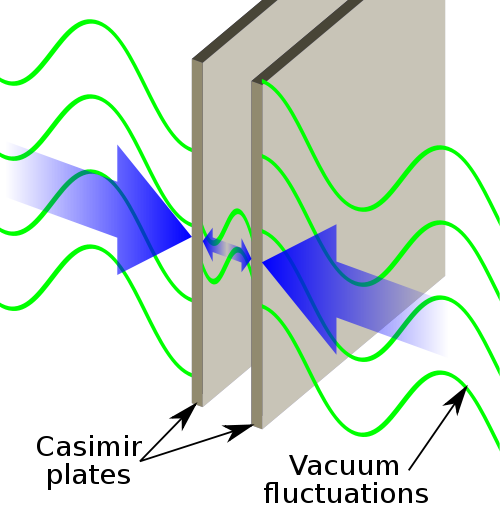
\includegraphics[width=\linewidth]{casimir.png}
\end{figure}

\end{column}
\end{columns}

\end{frame}


%------------------------------------------------
\section{Uniqueness}
%------------------------------------------------

\begin{frame}
\frametitle{Uniqueness} 
\begin{figure}

\includegraphics[width=0.55\linewidth]{unique.jpeg}
\end{figure}
\end{frame}

%------------------------------------------------

\subsection{Analytic Continuation}

\begin{frame}
\frametitle{Going Above and Beyond}

\begin{block}{Analytic Function}
An analytic function is an infinitely differentiable function such that its Taylor series converges pointwise in the domain. 
\end{block}

\begin{block}{Analytic Continuation}
Analytic continuation is a technique to extend the domain of a given analytic function while remain analytic. If an analytic continuation exists, it is guaranteed to be unique. Therefore, surprisingly, knowing the value of a complex function in some finite complex domain uniquely determines the value of the function at every other point.
\end{block}

\end{frame}

%------------------------------------------------

\subsection{Riemann Zeta Function}

\begin{frame}
\frametitle{Analytic Continuation of Euler Zeta Function}

Amazing video from 3Blue1Brown: \href{https://www.youtube.com/watch?v=sD0NjbwqlYw}{Visualizing the Riemann hypothesis and analytic continuation}. (9 min 40 s -- 17 min 20 s) \\ 

\begin{itemize}
    \item Euler established that 
    $$ E(s) = \sum_{n=1}^{\infty} \frac{1}{n^s} = \sum_{n=1}^{\infty} n^{-s} $$
    converges in Cauchy sense for $ \forall s > 1 $ \\ 
    (Hint: easy check using integral test.)
    \item Riemann treated it as a complex function and found its analytic continuation $\zeta$ which satisfies the functional equation 
    $$ \zeta(s) = 2^s \pi^{s-1} \sin \big( \frac{\pi s}{2} \big) \Gamma (1-s) \zeta(1-s) $$
\end{itemize}

\end{frame}

%------------------------------------------------

\begin{frame}
\frametitle{Sum of All Natural Numbers}

To find the sum of all natural numbers, it remains to find $\zeta(-1)$, 
$$ \zeta(-1) = 2^{-1} \pi^{-2} \sin \big( -\frac{\pi}{2} \big) \Gamma (2) \zeta(2) = - \frac{1}{2 \pi^2} \zeta(2) $$
where 
\begin{itemize}
    \item $\Gamma(n) = (n-1)!$ for $ \forall n \in \mathbb{N} $, hence $ \Gamma(2) = 1 $
\end{itemize}

We will now compute $\zeta(2)$, i.e. $E(2)$, which is convergent in Cauchy sense 

$$ \zeta(2) = \sum_{n=1}^{\infty} \frac{1}{n^2} = 1 + \frac{1}{4} + \frac{1}{9} + \frac{1}{16} + \cdots $$

\end{frame}

%------------------------------------------------

\begin{frame}
\frametitle{Basel Problem: $ \zeta(2) = E(2) = \frac{\pi^2}{6} $}
Consider $ p(x) = \frac{\sin(x)}{x} $, 
\begin{itemize}
    \item Power Series Expansion
    $$ p(x) = 1 - \frac{x^2}{3!} + \frac{x^4}{5!} - \frac{x^6}{7!} + \cdots = \sum_{n=0}^{\infty} (-1)^n \frac{x^{2n}}{(2n+1)!} $$ 
    \item Factorization (Formally, Weierstrass Factorization Theorem)
    \begin{align*}
        p(x) &= \big(1 - \frac{x}{\pi}\big)\big(1 + \frac{x}{\pi}\big)\big(1 - \frac{x}{2\pi}\big)\big(1 + \frac{x}{2\pi}\big)\big(1 - \frac{x}{3\pi}\big)\big(1 + \frac{x}{3\pi}\big)\cdots \\ 
        &= \prod_{n=1}^{\infty} \big(1 - \frac{x^2}{n^2 \pi^2}\big) 
        = 1 - \big( \frac{1}{\pi^2} + \frac{1}{4\pi^2} + \frac{1}{9\pi^2} + \cdots \big) x^2 + \cdots 
    \end{align*}
\end{itemize}

\end{frame}

%------------------------------------------------

\begin{frame}
\frametitle{Basel Problem: $ \zeta(2) = E(2) = \frac{\pi^2}{6} $ (Cont.)}

The two expression of $p(x)$ must match, i.e. coefficients for each $x^k$ power mush agree. In particular, let's look at coefficients for $x^2$ term. (This method works for any even order. Euler obtained up to 26.)

\begin{align*}
    -\frac{1}{3!} &= - \big( \frac{1}{\pi^2} + \frac{1}{4\pi^2} + \frac{1}{9\pi^2} + \cdots \big) \\ 
    -\frac{1}{6}  &= - \frac{1}{\pi^2} \sum_{n=1}^{\infty} \frac{1}{n^2} \\ 
    \implies \sum_{n=1}^{\infty} \frac{1}{n^2} &= \frac{\pi^2}{6}
\end{align*}

Consequently, we have \alert{ $ \zeta(-1) = -\frac{1}{12} $ }

\end{frame}

%------------------------------------------------

\begin{frame}
\frametitle{Bonus: Riemann Hypothesis}

Euler showed that (now known as Euler Product Formula)
$$ \zeta(s) 
= \prod_{p \text{ prime}} \frac{1}{1 - p^{-s}} 
= \frac{1}{1 - 2^{-s}} \cdot \frac{1}{1 - 3^{-s}} \cdot \frac{1}{1 - 5^{-s}} \cdot \cdots $$

In regards to zeros, Riemann hypothesized, for $ \forall s \in \mathbb{C} $ s.t. $ \zeta(s) = 0 $
\begin{itemize}
    \item Either, $ s = -2n $ for some $ n \in \mathbb{N} $, known as \emph{trivial zeros} 
    \item Or, $ \text{Re}(s) = \frac{1}{2} $, forming a \emph{critical line}
\end{itemize}

\end{frame}

%------------------------------------------------

\section*{}
\begin{frame}
\Huge{\centerline{Questions?}}
\end{frame}

%----------------------------------------------------------------------------------------

\end{document}